\documentclass[a4paper, 12pt]{article}
\usepackage{cmap}
\usepackage[utf8]{inputenc}
\usepackage[english, russian]{babel}
\usepackage[left=2cm, right=2cm, top=2cm, bottom=2cm]{geometry}
\usepackage{amsfonts,amssymb}
\usepackage{amsmath}
\usepackage{amsthm}
\usepackage{titlesec}
\usepackage{graphicx}
\usepackage{mathtools}
\usepackage{hyperref}

 \newcommand{\tit}[1]{\begin{center}{\bf{\Large #1}}\end{center}}
 \newcommand{\aut}[1]{\centerline{{\bf #1}}}
 \newcommand{\cityorg}[1]{\centerline{\it #1}}
 \newcommand{\email}[1]{\centerline{{\small e-mail: #1}}\vspace{\baselineskip}}
\providecommand{\keywords}[1]{\textbf{\textit{Ключевые слова:}} #1}
\newcommand{\norm}[1]{\left\lVert#1\right\rVert}
\newcommand{\normb}[1]{\left\lVert\textbf{#1}\right\rVert}

\begin{document}

\sloppy

 \tit{Идеальная цилиндрическая оболочка: совершенная, но чувствительная к малым возмущениям}
 \tit{Ideal Cylindrical Cloak: Perfect but Sensitive to Tiny Perturbations}
 \aut{Zhichao Ruan, Min Yan, Curtis W. Neff, and Min Qiu}
 \cityorg{Laboratory of Optics, Photonics and Quantum Electronics,} 
 \cityorg{Department of Microelectronics and Applied Physics,} 
 \cityorg{Royal Institute of Technology (KTH), Electrum 229, 16440 Kista, Sweden}
 \cityorg{Joint Research Center of Photonics of the}
 \cityorg{Royal Institute of Technology (Sweden) and Zhejiang University,}
 \cityorg{Zhejiang University, Yu-Quan, 310027 Hangzhou, People’s Republic of China}
 \email{min@kth.se}

\begin{abstract}
Метод разложения цилиндрической волны разработан для получения рассеяния для идеальной двумерной цилиндрической
маскирующей оболочки.Почти идеальная модель маскирующей оболочки настроена, чтобы решить краевую задачу на внутренней
грнице оболочки. Систематически изучив изменение коэффициентов рассеяния от почти идеального случая до идеального, мы
подтверждаем, что оболочка с идеальными физическими параметрами является совершенной маскируюущей оболочкой. Но из-за
медленной сходимости коэффициентов рассеяния, малые возбуждения на оболочке индуцируют заметное рассеяние и проникновение
поля. Мы также доказали, что рассеянные и проникшие поля доминируются цилиндрическими волнами нулевого порядка. Хотя
наша работа была сосредоточена на двумерной оболочке, она может быть обобщена на трехмерный случай. 
\end{abstract}

В последних работах обсуждался захватывающий вопрос экзотичесих материалов, невидимых для электромагнитных волн
(EM) \cite{1}-\cite{11}. Основываясь на преобразовании координат в уравнениях Максвелла Пендри и другие впервые
предложили мантию невидивку, которая может защищать объект внутри нее от обнаружения \cite{1}: когда 
электромагнитные волны проходят сквозь мантию невидимку, она отражает их, направляя вокруг объекта, затем
возвращает в первоначальное направление, не возмущая внешнее поле. Также недавно сообщалось о численных методах,
примененных для решения задачи EM, включающаю маскирующую оболочку \cite{6,9}, и экспериментальных результатов 
маскировки с использованием метаматериалов с упрощенными параметрами \cite{7}. Тем не менее, идеальная маскирующая 
оболочка не была подтверждена как совершенная оболочка, в связи с экстримальными физическими параметрами (ноль 
или бесконечность) в идеальной оболочке при приближении к внутренней границе.

В этой работе мы рассмотрим рассеяние идеальной маскирующей оболочки.
Мы сфокусируем наш анализ на двумерной циллиндрической
оболочке, поскольку волновое уравнение, по сравнению с трехмерным случаем может быть упрощено, так же двумерную оболочку
более проще изготовить \cite{7}. Мы воспользуемся приемуществом цилиндрической геометрии структуры и используем
метод разложения в ряд цилиндрической волны для изучения устройства полуаналитически. Чтобы избежать экстремальных значений
(нуля или бесконечности), мы введем небольшое возмущение в идеальную оболочку и позволим ему достигнуть нуля, чтобы
изучить задачу рассеяния для идеальной оболочки. Такой асимптотический анализ может показать не только, является ли
идеально невидимой или нет, но и предоставляет подсказки, насколько чувствительно такое устройство к конечным 
возмущениям. Анализ чувствительности оболочки прямо определяет возможно его применения. Наши исследования 
показывают, что цилиндическая оболочка очень чувствительна к малым возмущениям параметров.

Сначала посмотрим на волновое уравнение внутри цилиндрической оболочки. Согласно \cite{1} простое преобразование

\begin{equation}\label{e1}
	r' = \frac{b-a}{b}r+a, \;\; \theta' = \theta, \;\; \zeta' = \zeta
\end{equation}
может сжать пространство из цилиндрической области $0 < r < b$ в кольцо $0 < r' < b$, где $a$ и $b$ внутренний и
внешний радиусы оболочки соответственно, и $r, \theta, \zeta (r', \theta', \zeta')$ радиальная, угловая и вертикальная
координаты в оригинальной(преобразованной) системе соответственно. Следуя подходу работы \cite{1} компоненты тензора 
диалектрическая и магнитая проницаемости могут быть записаны как 

\begin{equation*}
	\varepsilon_r = \mu_r = \frac{r-a}{r} \;\;\; \varepsilon_\theta = \mu_\theta = \frac{r}{r-a},	
\end{equation*}  

\begin{equation}\label{e2}
	\varepsilon_\zeta = \mu_\zeta = (\frac{b}{b-a})^2 \frac{r-a}{r}
\end{equation}
и предполагается воздух для окружающей среды и внутренней области. В дальнейшем рассматривается 
поперечно-электрическое(TE) полязированное магнитное поле (т.е. электрическое поле существует только в 
$\zeta$-направлении); однако, аналогичные рассуждения могут быть проведены для поперечно-магнитного поля. На протяжении
работы предполагается $\exp(-iwt)$ зависимость от времени. Для TE-поляризованной волны только $\varepsilon_\zeta, \mu_r$
и $\mu_\theta$ относятся к следущему общему волновому уравнению, регулирующему поле $\textbf{E}_\zeta$ в цилиндрических 
координатах оболочки

\begin{equation}\label{e3}
	\frac{1}{\varepsilon_\zeta r} \frac{\partial}{\partial r}(\frac{r}{\mu_\theta}\frac{\partial \textbf{E}_\zeta}
	{\partial r}) +
	\frac{1}{\varepsilon_\zeta r^2} \frac{\partial}{\partial \theta}(\frac{1}{\mu_r}\frac{\partial \textbf{E}_\zeta}
	{\partial \theta}) + k_0^2 \textbf{E}_\zeta = 0,
\end{equation}
где $k_0$ волновой вектор света в вакууме. Если мы подставим ур. \eqref{e2} для $\varepsilon_\zeta, \mu_r$ и 
$\mu_\theta$ получим
\begin{equation}\label{e4}
	r^2 \frac{\partial^2 \textbf{E}_\zeta}{\partial r^2} + r\mu_\theta \frac{\partial \textbf{E}_\zeta}{\partial r} + 
	\varepsilon_\zeta \mu_\theta r^2 k_0^2 \textbf{E}_\zeta + \frac{\mu_\theta}{\mu_r} \frac{\partial^2 
	\textbf{E}_\zeta}{\partial \theta^2} = 0.
\end{equation}
Уравнение \eqref{e4} может быть решено разделением переменных
$ \textbf{E}_\zeta = \mathbf{\Psi}(r) \mathbf{\Theta}(\theta)$ и введением константы $l$:
\begin{equation}\label{e5}
	(r-a)^2 \frac{\partial^2 \mathbf{\Psi}}{\partial r^2} + (r-a) \frac{\partial \mathbf{\Psi}}{\partial r} +
	\left[ (\frac{b}{b-a})^2(r-a)^2 k_0^2-l^2\right] \mathbf{\Psi} = 0,
\end{equation}

\begin{equation}\label{e6}
	\frac{\partial^2 \mathbf{\Theta}}{\partial \theta^2} + l^2 \mathbf{\Theta} = 0.
\end{equation}
Уравнение \eqref{e5} есть диффиренциальное уравнение Бесселя порядка $l$, а общее решение ур. \eqref{e6} имеет вид
$\exp(il\theta)$. Поэтому существует простое множество решений $\mathbf{E}_\zeta$ в маскирующей оболочке вида

\begin{equation}\label{e7}
	F_l(k_1(r-a))\exp(il\theta),
\end{equation}
где $k_1 = k_0 b/(b-a), F_l$ функция Бесселя порядка $l$, $l$ --- целое число, как того требует вращательное граничное 
условие.

Рассмотрим задачу рассеяния, в которой произвольная волна падает на оболочку. Согласно строгой теории рассеяния 
\cite{12}, падающее поле в двумерном случае может быть разложено по координатам оболочки следущим образом:

\begin{equation}\label{e8}
	\mathbf{E}_\zeta^{in} = \sum\limits_l \alpha_l^{in} \mathbf{J}_l(k_0 r)\exp(il\theta),
\end{equation}
где $\mathbf{J}_l$ функция Бесселя порядка $l$ первого рода. Рассеянное поле так же может быть разложено как

\begin{equation}\label{e9}
	\mathbf{E}_\zeta^{sc} = \sum\limits_l \alpha_l^{sc} \mathbf{H}_l(k_0 r)\exp(il\theta),
\end{equation}
где $\mathbf{H}_l$ функция Ханкеля порядка $l$ первого рода.

\begin{figure}[t]
  \centering
  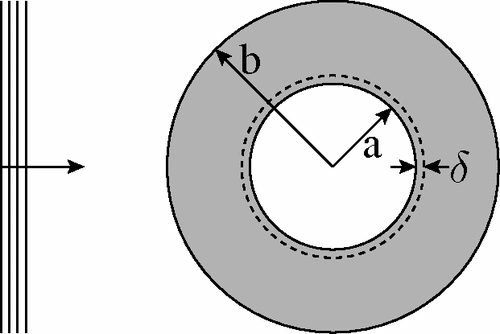
\includegraphics[height=0.15\paperheight]{1.png}
  \caption{Схема почти идеальной маскировочной оболочки: распределение параметров такое же, как идеальное, показанное в
  ур. \eqref{e2} и внешняя граница зафиксирована в $r=b$. Однако реальная внутренняя граница расположена в 
  $r=a +\delta$, где $\delta$ очень маленькое положительное число.}
  \label{fig:1}
\end{figure}

Отметим, что коэффициенты рассеяния не могут быть прямо получены для идеального плаща, так как $\varepsilon_\zeta \to 0,
\mu_r \to 0$ и $\mu_\theta \to \infty$, когда $r \to a$, и функции Бесселя второго рода в ур. \eqref{e7} имеют 
сингулярность при $r = a$. Чтобы обойти это мы вводим малое возмущение в идеальную оболочку, на такую оболочку будем
ссылаться как на почти идеальную, см. Рис.\ref{fig:1}.  Мы немного расширим внутреннюю границу так, что она будет
находится в $r = a + \delta$, где $\delta$ очень маленькое положительное число. Тем не менее, параметры все еще
вычисляются согласно формуле \eqref{e2}, как будто внутренняя граница не поменялась. Внешняя граница остается
зафиксированной $r = b$. Когда $\delta \to 0$ наша модель будет эквивалентна идеальной оболочке. Теперь электрическое
поле в каждой области задается соотношениями

\begin{equation*}
	(b<r)\mathbf{E}_\zeta = \sum\limits_l (\alpha_l^{in} \mathbf{J}_l(k_0 r)\exp(il\theta) +
								\alpha_l^{sc} \mathbf{H}_l(k_0 r)\exp(il\theta))
\end{equation*}
 
\begin{equation}\label{e10}
	(a+\delta<r<b)\mathbf{E}_\zeta = \sum\limits_l (\alpha_l^{1} \mathbf{J}_l(k_0 (r-a))\exp(il\theta) +
								\alpha_l^{2} \mathbf{H}_l(k_0 (r-a))\exp(il\theta))
\end{equation}

\begin{equation*}
	(r<a+\delta)\mathbf{E}_\zeta = \sum\limits_l \alpha_l^{3} \mathbf{J}_l(k_0 r)\exp(il\theta)
\end{equation*}
где $\alpha_l^i(i=1,2,3)$ коэффциенты разложения для результирующего поля внутри оболочки.

Касательные поля $\mathbf{E}_\zeta$ и $\mathbf{H}_\theta$(которое может быть получено из $\mathbf{E}_\zeta$)
должны быть непрерывны вдоль границы $r=a+\delta$ и $r=b$ и ортогональность $\exp(il\theta)$ позволяет волнам
в каждом порядке Бесселя разделяться. Таким образом, имеем следущие четыре уравнения:

\begin{equation}\tag{11a}\label{e11a}
	\alpha_l^{in} \mathbf{J}_l(k_0 b) + \alpha_l^{sc} \mathbf{H}_l(k_0 b) = 
	\alpha_l^1 \mathbf{J}_l(k_1(b-a)) + \alpha_l^2 \mathbf{H}_l(k_1(b-a)) 	
\end{equation}

\begin{equation}\tag{11b}\label{e11b}
	\alpha_l^1 \mathbf{J}_l(k_1 \delta) + \alpha_l^2 \mathbf{H}_l(k_1 \delta) = \alpha_l^3 \mathbf{J}_l(k_0(a+\delta)) 
\end{equation}

\begin{equation}\tag{11c}\label{e11c}
	k_0\alpha_l^{in} \mathbf{J}'_l(k_0 b) + \alpha_l^{sc} \mathbf{H'}_l(k_0 b)	=
	\frac{k_1}{\mu_\theta(b)} \alpha_l^1 \mathbf{J'}_l(k_1(b-a)) + \frac{k_1}{\mu_\theta(b)} \alpha_l^2 \mathbf{H'}_l
	(k_1(b-a)) 	
\end{equation}

\begin{equation}\tag{11d}\label{e11d}
	\frac{k_1}{\mu_\theta(a+\delta)}\alpha_l^1 \mathbf{J'}_l(k_1 \delta) + \frac{k_1}{\mu_\theta(a+\delta)}
	\alpha_l^2 \mathbf{H'}_l(k_1 \delta) = k_0\alpha_l^3 \mathbf{J'}_l(k_0(a+\delta)),
\end{equation}
которые являются линейными. При этом каждый коэффициент разложения в каждой существенной области может быть точно решен.
В свою очередь, в каждой области мы можем получить поля.

\begin{figure}[t]
  \centering
  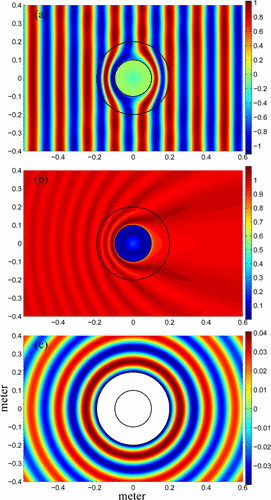
\includegraphics[height=0.3\paperheight, width=0.22\paperwidth]{2.png}
  \caption{(a)Снимки результирующего распределения электрического поля (b) соответствующая норма в непосредственной 
  близости к маскируемому объекту (c)снимок соответствуюущего рассеянного поля вне оболочки для почти идеальной маскировки
  с $\delta = 10^{-5}a$, когда плоская волная падает на оболочку перпендикулярно. Черные линии обозначают оболочку, еденицы
  измерения осей: метры}
  \label{fig:2}
\end{figure}

Прямо из этой системы линейных уравнений можно показать, что когда $\delta \to 0, \alpha_l^{sc}=\alpha_l^{2} \to 0, 
\alpha_l^1=\alpha_l^{in}$ и $\alpha_l^3 \to 0$ для любого $\alpha_l^{in}$, т.е. идеальная оболочка есть совершенная 
маскирующая оболочка. Во первых, можно предположить, что $\left| \alpha_l^i(i=sc,1,2,3) \right|$ должны быть конечны.
В противном случае рассеянное поле будет бесконечным, если входящее поле будет иметь компоненту порядка $l$. Во вторых,
когда $\delta \to 0, k_1(b-a)=k_0 b$ и $k_1=k_0 \mu_\theta(b)$ ур. \eqref{e11a} и \eqref{e11c} становятся 
$(\alpha_l^{in}-\alpha_l^1)\mathbf{J}(k_0 b) + (\alpha_l^{sc}-\alpha_l^2)\mathbf{H}_l(k_0 b) = 0$ и 
$(\alpha_l^{in}-\alpha_l^1)\mathbf{J'}(k_0 b) + (\alpha_l^{sc}-\alpha_l^2)\mathbf{H'}_l(k_0 b) = 0$ соответственно.
Так как $b$ может быть произвольным и функции Бесселя не всегда равны нулю должно выполняться $\alpha_l^{in}=\alpha_l^1$ и
$\alpha_l^{sc}=\alpha_l^2$. В третьих из ур. \eqref{e11b} можно получить следущее неравенство:

\stepcounter{equation}

\begin{equation}\label{e12}
	\left| \alpha_l^2\mathbf{H}(k_1 \delta) \right| \le \left| \alpha_l^3 \mathbf{J}_l(k_0(a+\delta)) \right| + 
	\left| \alpha_l^1 \mathbf{J}_l(k_1 \delta) \right|. 
\end{equation}
Когда $\delta \to 0$ правая часть неравенства приближается к конечному числу, но $\left| \mathbf{H}(k_1 \delta) \right|$ 
приближается к бесконечности. Тоесть $\left| \alpha_l^2 \right|$ должно стремиться к нулю. Наконец, из уравнения 
\eqref{e11b} можно получить $\left| \alpha_l^2 \mathbf{H'}_l(k_1 \delta) \right| \le \left| \alpha_l^3 \frac{k_0}{k_1}
\mathbf{J'}_l(k_0(a+\delta))\right|+\left| \alpha_l^1\mathbf{J'}_l(k_1 \delta)\right|$. В то время как из ур. \eqref{e11d} 
имеем

\begin{equation}\label{e13}
	\left| k_0 \alpha_l^3 \mathbf{J'}_l(k_0(a+\delta))\right| \le
	\left| \frac{k_1}{\mu_\theta(a+\delta)}\alpha_l^1 \mathbf{J'}_l(k_1 \delta) \right| + 
	\left| \frac{k_1}{\mu_\theta(a+\delta)}\alpha_l^2 \mathbf{H'}_l(k_1 \delta) \right|
\end{equation}
Так как $\mu_\theta(a+\delta) \to \infty$ и правая часть неравенства стремится к нулю, когда $\delta \to 0$, получаем
$|\alpha_l^3| \to 0$. Это рассуждение показывает, что рассеянное поле и поле внутри оболочки равны нулю, когда $\delta=0$,
тоесть идеальная оболочка есть совершенная маскирующая оболочка.

\begin{figure}[t]
  \centering
  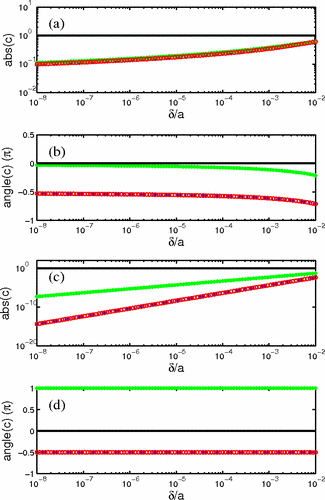
\includegraphics[height=0.3\paperheight, width=0.26\paperwidth]{3.png}
  \caption{Амплитуда и фаза коэффициентов рассеяния для различных $\delta$, где $(a),(b)$ и $(c),(d)$ отвечают случаям 
  $l=0$ и $l=1$ соответсвенно. $c_l^{sc}$ обозначено синим, или темно-серой штрихованной линией, $c_l^{1}$ обозначено
  черной линией, $c_l^2$ красной или серой линией с кружочками, и $c_l^3$ зеленая или светло-серая линия звездочками}
  \label{fig:3}
\end{figure}

Хотя мы только что подтвердили, что идеальная оболочка может осуществлять совершенную маскировку, дальнейшее изучение
указанным выше аналитическим методом почти идеальной оболочки показывает, насколько чувствителен параметр $\delta$ к 
производительности оболочки. Как пример мы используем те же параметры в \cite{6}, в которой внутренний радиус $a=0.1м$,
внешний радиус оболочки $b=0.2m$ и частота падающей плоской волны $2ГГц$. Аналогично, мы также рассматриваем плоскую
падающую волну, а коэффициенты разложения в ур. \eqref{e8} равны
 
\begin{equation}
	\alpha_l^{in} = i^l A \exp(-ik_0r_1\cos(\varphi+\theta_1)-il\varphi),
\end{equation}
где $(r_1, \theta_1, 0)$ координаты точки опорной фазы, А --- амплитуда плоской волны и $\varphi$ угол падения \cite{13}.
Здесь точка опорной фазы установлена в $r_1=4a$ и $\theta_1=\pi$, амплитуда $A=1$ и угол падения $\varphi=0$(тоесть 
плоская волна распостраняется слева на право). Мы использовали 31 член Бесселя ($-15 \le l \le 15$) чтобы посчитать
рассеянное поле для почти идеальной оболочки с $\delta=10^{-5}a$. Количество взятых членов разложения достаточно для
сходимости вычисленных полей. Рис. (\ref{fig:2}) показывает снимок результирующего распределния электрического поля(т.е. 
вещественную часть комплескного электрического поля) и соответствующую норму в непосредственной близости к маскируемуму 
объекту. Распределениеиэлектрического поля ясно показывает эффект маскировки на почти идеальной оболочке для плоской
падающей волны. Тем не менее, норма электрического поля на рис.(\ref{fig:2}b) показывает, что немного поля находится в
внутрени оболочки и присутствует очевидная рябь рассеяния вокруг оболочки. Амлитуда результурующего электрического поля
в центре равна $0.197$. Снимок рассеянного поля на рис. (\ref{fig:2}c) показывает, что оно распостраняется почти изотропно
во всех углах. Даже несмотря на то, что амплитуда рассеянного поля гораздо меньше, чем амплитуда падающей волны, 
интерференция падающей плоской волны и рассеянного поля создает рябь в норме, рис. (\ref{fig:2}b).

Так как каждый коэффициен разложения рассеянного поля соответствует коэффициенту входящего поля (сравни с ур.(11)), мы
можем определить коэффициент рассеяния для каждого порядка как

\begin{equation}
	c_l^{sc} = \frac{\alpha_l^{sc}}{\alpha_l^{in}}.
\end{equation}
Эти коэффициенты для полей внтури оболочки $c_l^{(i)}= \alpha_l^{i}/\alpha_l^{in}, i=1,2,3$ могут быть определены таким же
образом. Для изучения идеальной оболочки мы сдвинем $\delta$ ближе к нулю. Амплитуда и фаза этих коэффициентов для
$10^{-8}a<\delta<10^{-2}a$ показаны на рис. (\ref{fig:3}), где $(a),(b)$ и $(c),(d)$ отвечают случаям $l=0$ и $l=1$
соответсвенно.

Из рис. \ref{fig:3} ясно, что $c_l^{(1)}$ всегда равно 1 для обоих случаев. То есть падающее поле распостраняется в 
оболочке без отражения на внешней границе, что совпадает с объяснением эффекта маскивроки для подхода преобразования 
координат \cite{1}. Такое же поведение для рассеянных полей возникает на внешней границе, где они распостраняются 
изнутри наружу без отражений, таким образом $c_l^{sc}$ всегда равно $c_l^2$.

Наши вычислительные результаты также подтверждают, что оба $c_l^{sc}$ и $c_l^3$ стремятся к нулю, когда $\delta \to 0$.
В частности, по сравнению с случаем $l=0$, $|c_l^{sc}|$ и $|c_l^3|$ намного меньше, для $l=1$, и прибижаются к нулю гораздо
быстрее. Также это наблюдается для случаев с более высоким порядком. Поэтому, в случае плоской волны, в котором 
$|\alpha_l^{in}|$ одинаковы для всех порядков, доминантные члены рассеянного поля имебт вид функций Ханкеля нулевого 
порядка первого рода. В то же время, результирующее поле в внутренней области имиет доминирубщий член $\mathbf{J}_0(k_0r)$.
Это объясняет неизменное распределение поля возле азимута в внутренней области (см. рис.\ref{fig:2}a) и рассеянное поле 
вне оболочки (см. рис. \ref{fig:2}b), что также упомянуто в \cite{6}.

Стоит отметить, что коэффициенты рассеяния нулевого порядка $c_0^{sc}$ и $c_0^{(3)}$ крайне медленно убывают с уменьшением
$\delta$; т.е., когда $\delta$ уменьшеается с $10^{-5}a$ до $10^{-8}a$, $|c_0^{sc}|$ уменьшается только с $0.175$ до 
$0.099$. При использовании произвольной точности программного обеспечения MATHEMATICA, что сходимость предела настолько
медленная, что даже при $\delta = 10^{-99}a$(т.е. $\varepsilon \approx 4 \times 10^{-99}, \mu_r \approx 10^{-99}$ и 
$\mu_\theta 10^{99}$ на внутренней границе в этом случае), $|c_l^{sc}| = 6.973 \times 10^{-3}$. Таким образом мы приходим
к выводу, что хотя оболочка с идеальными параметрами в \cite{1} совершенная оболочка, неидеальная оболочка не обеспечивает
достаточно хороший эффект маскировки из-за медленной сходимости $|c_0^{sc}|$ и $|c_0^{(0)}|$.

В заключение, мы использовали метод разложения в ряд цилиндрической волны для изучения электромагнитных свойств двумерной
маскирующей оболочки. Почти идеальная модель маскирующей оболочки настроена, чтобы решить краевую задачу на внутренней
грнице оболочки. Систематически изучив изменение коэффициентов рассеяния от почти идеального случая до идеального, мы
подтверждаем, что оболочка с идеальными физическими параметрами является совершенной маскируюущей оболочкой. Но из-за
медленной сходимости коэффициентов рассеяния, малые возбуждения на оболочке индуцируют заметное рассеяние и проникновение
поля. Мы также доказали, что рассеянные и проникшие поля доминируются цилиндрическими волнами нулевого порядка. Хотя
наша работа была сосредоточена на двумерной оболочке, она может быть обобщена на трехмерный случай. Наши методы и 
результаты могут быть использованы для обнаружения и проектирования маскирующей оболочки такого типа.

\begin{thebibliography}{99}
\bibitem{1}J. B. Pendry, D. Schurig, and D. R. Smith, Science 312, 1780 (2006).
\bibitem{2}U. Leonhardt, Science 312, 1777 (2006).
\bibitem{3}A. Alu and N. Engheta, Phys. Rev. E 72, 016623 (2005).
\bibitem{4}D. A. B. Miller, Opt. Express 14, 12457 (2006).
\bibitem{5}U. Leonhardt, New J. Phys. 8, 118 (2006).
\bibitem{6}S. A. Cummer, B. I. Popa, D. Schurig, D. R. Smith, and J. B. Pendry, Phys. Rev. E 74, 036621 (2006).
\bibitem{7}D. Schurig, J. J. Mock, B. J. Justice, S. A. Cummer, J. B. Pendry, A. F. Starr, and D. R. Smith, 
Science 314, 977 (2006).
\bibitem{8}G. W. Milton, M. Briane, and J. R. Willis, New J. Phys. 8, 248 (2006).
\bibitem{9}F. Zolla, S. Guenneau, A. Nicolet, and J. B. Pendry, Opt. Lett. 32, 1069 (2007).
\bibitem{10}W. Cai, U. K. Chettiar, A. V. Kildishev, and V. M. Shalaev, Nat. Photon. 1, 224 (2007).
\bibitem{11}H. Chen and C. T. Chan, Appl. Phys. Lett. 90, 241105 (2007).
\bibitem{12}H. C. van de Hulst, Light Scattering by Small Particles(Dover, New York, 1981).
\bibitem{13}D. Felbacq, G. Tayeb, and D. Maystre, J. Opt. Soc. Am. A 11, 2526 (1994).
\end{thebibliography}

\end{document}
